
The tool is highly configurable and it is possible to create own plugins or add new tests in the configuration files without having any development experience. As it is aligned with modern security standards, these standards should be introduced in the following sub sections.

\subsection{OWASP Top 10}

The Open Web Application Security Project (OWASP) is a non-profit foundation dedicated to improving the security of software. The \textbf{OWASP Top 10} is a standard awareness document for developers and web application security. It represents a broad consensus about the most critical security risks to web applications (\cite{Top10.11.06.2021}). It defines the top 10 most critical web application security risks, based on a consensus from security experts around the world. Every 2-3 years the list is updated according to changes related the field of security. \ac{owtf} contains plugins for each of these vulnerabilities.

\subsection{OWASP Web Security Testing Guide}

The \textbf{OWASP Testing Guide} (current iteration: v4) is a comprehensive guide related testing the security of web services and applications (\cite{Guide.11.06.2021}). It gives developers, testers and management a structured approach for questions like "When, Why \& What to test" - specifically related to the \ac{sdlc}. Lots of plugins from \ac{owtf} are directly aligned to the tests defined in this guide.

\subsection{Penetration Testing Execution Standard}

The \ac{ptes} (\cite{PTES.11.06.2021}) is a standard which defines the process of penetration testing. It is structured into 7 phases: 

\begin{enumerate}
	\item Pre-engagement Interactions
	\item Intelligence Gathering
	\item Threat Modeling
	\item Vulnerability Analysis
	\item Exploitation
	\item Post Exploitation
	\item Reporting
\end{enumerate}

\ac{owtf} is trying to follow this standard and all of its phases.

\subsection{NIST SP 800-115}

The SP 800-115 Technical Guide to Information Security Testing and Assessment from the \ac{nist} is a guide to the basic technical aspects of conducting information security assessments \cite{NIST.29.06.2021}. Some plugins from \ac{owtf} are also directly aligned to the tests defined in this guide.

\section{Features}

Some features provided by the tool:

\begin{itemize}
	\item Resilience: If one plugin/command crashes, the tool will move on to the next
	\item Tests Separation
	\begin{itemize}
		\item Passive : No traffic goes to the target
		\item Semi Passive : Normal traffic to target
		\item Active: Direct vulnerability probing
	\end{itemize}
	\item Extensive REST API
	\item Aligned with OWASP Testing Guide(v3, v4), Top 10
	\item Simple intuitive web interface: manage large penetration engagements easily
	\item Report generation and export
\end{itemize}

\subsection{Workflow}

\begin{figure}[H]
	\centering
	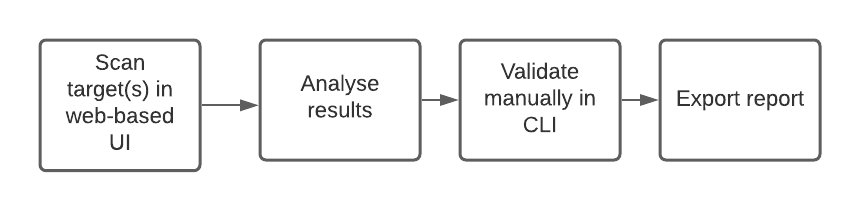
\includegraphics[width=12cm,keepaspectratio=true]{pictures/workflow1.png}
	\caption{
		Workflow (\cite{Brennen.11.06.2021})
	}
	\label{fig:workflow1}
\end{figure}

As shown in figure \ref{fig:workflow1}, the basic workflow for usage of the tool is pretty straightforward:

\begin{enumerate}
	\item Add target URL(s)
	\item Run plugins
	\item Analyse scan results
	\item Copy commands from web UI to CLI
	\item Run CLI commands
	\item Analyse/verify the CLI results
	\item Add notes in the web UI
	\item Generate (export) the report
\end{enumerate}


\section{Technical analysis}

This section gives a short overview of the technical specification, the tools running under the hood and the architecture of \ac{owtf}.

\subsection{Tech specs}

\begin{itemize}
	\item python 2.7
	\item PostgreSQL database backend
	\item Installation in Kali linux (docker available too)
	\item REST API
	\item web based user interface to control the tool
\end{itemize}

\subsection{Under the hood}

\begin{itemize}
	\item curl
	\item Arachni (\cite{Arachni.11.06.2021}) - feature-full, modular, high-performance Ruby framework aimed towards helping penetration testers and administrators evaluate the security of modern web applications
	\item w3af (\cite{WAF.11.06.2021}) - Web Applic^ation Attack and Audit Framework
	\item Skipfish (\cite{Skipfish.11.06.2021}) - active web application security reconnaissance tool
	\item DirBuster (\cite{DirBuster.11.06.2021}) - multi threaded java application designed to brute force directories
	\item Other well known tools like nmap, hydra, wpscan, whatweb, wapiti, metasploit, etc...
\end{itemize}

\subsection{Architecture}

\begin{figure}[H]
	\centering
	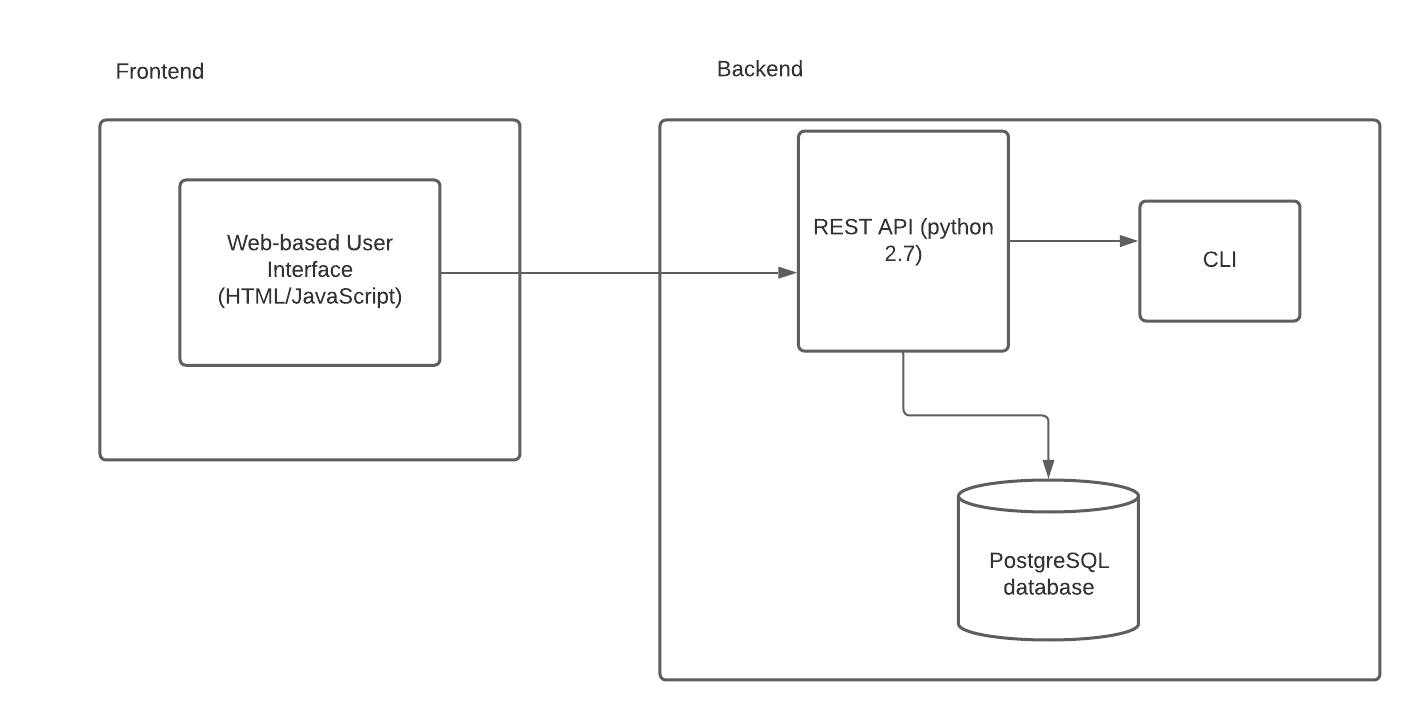
\includegraphics[width=12cm,keepaspectratio=true]{pictures/architecture.png}
	\caption{
		\ac{owtf} basic architecture diagram
	}
	\label{fig:architecture}
\end{figure}

As shown in figure \ref{fig:architecture}, basic architecture is split into a \textbf{Frontend}, containing a web based user interface for controlling and using the tool written in JavaScript using the popular React.js Framework from Facebook. A simple Express.js based server is responsible for serving the built assets to the client. The \textbf{Backend} implements a REST-based API written in python and communicates with a PostgreSQL database and the command line for executing different commands under the hood when the user runs plugins. 
It is possible to think of \ac{owtf} as a kind of collection of sophisticated tools for penetration testers, put together behind a nice user interface for controlling everything.


\section{Installation}

\begin{figure}[H]
	\centering
	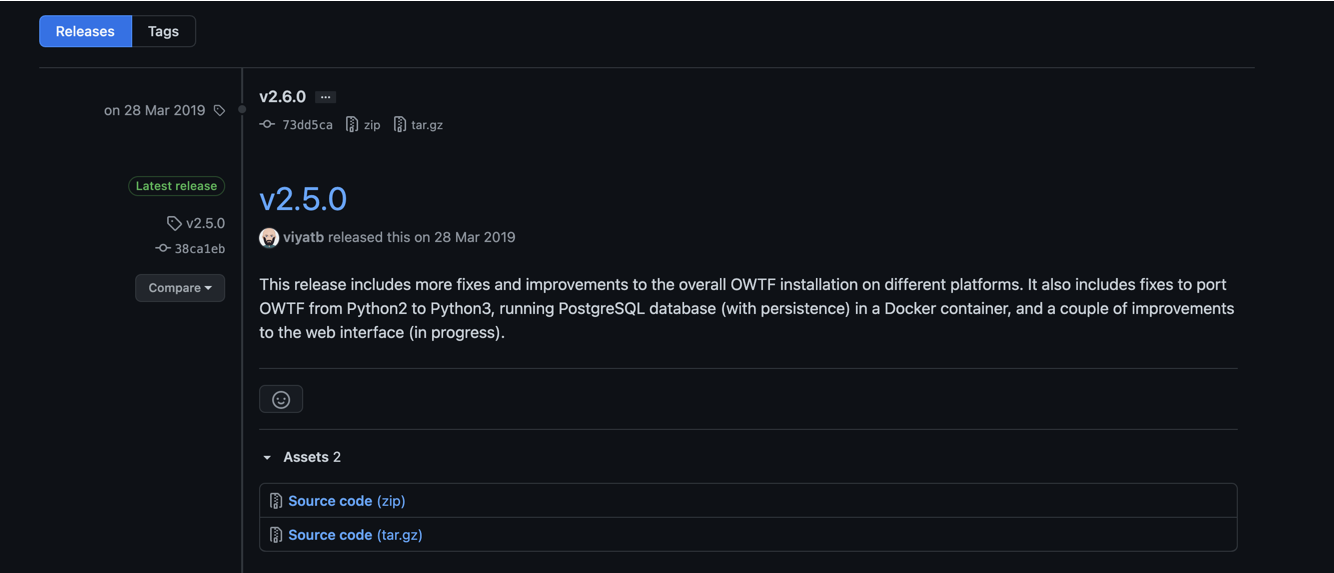
\includegraphics[width=12cm,keepaspectratio=true]{pictures/lastest-release.png}
	\caption{
		Latest release page on GitHub
	}
	\label{fig:lastest-release}
\end{figure}

It is possible to install all the dependencies on a kali linux machine, but the project repository also provides configuration files for a docker-based installation, so for reasons of simplicity the docker based installation will be used. Also the docker based installation is recommended by the contributors.

The latest official release of \ac{owtf} is from march 2019 as shown in figure \ref{fig:lastest-release}. Installing from docker in this release was not possible due to docker image authentication errors, so instead the latest state of the repository "develop" branch was used. Following the installation instructions from the official project README file, the installation routine using docker is quite simple and can be executed using the following commands:

\begin{lstlisting}
$ git clone https://github.com/owtf/owtf
$ cd owtf
$ make compose
\end{lstlisting}

The command \textbf{make compose} pulls a kali linux image and installs all the additional dependencies needed by the tool. After fetching and installing everything it finally starts the tool as shown in figure \ref{fig:docker-output}. Now the database is up and running, a proxy to the API and a webserver is listening for requests and the web based user interface can be accessed via a browser at the URL \textbf{http://localhost:8009/}.

\begin{figure}[H]
	\centering
	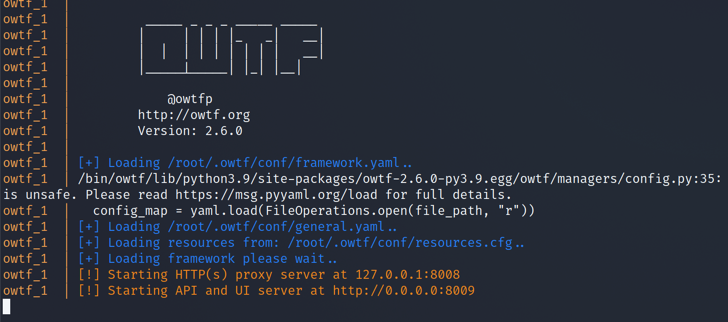
\includegraphics[width=12cm,keepaspectratio=true]{pictures/docker-output.png}
	\caption{
		OWTF startup terminal output
	}
	\label{fig:docker-output}
\end{figure}

\section{Usage}

The following sections will walk the reader through the different screens according to the workflow described above.

\subsection{User interface}

After installing and running the tool, the web based user interface is available and can be accessed via a web browser. First we want to add a target to scan.

\subsubsection{Adding targets}

\begin{figure}[H]
	\centering
	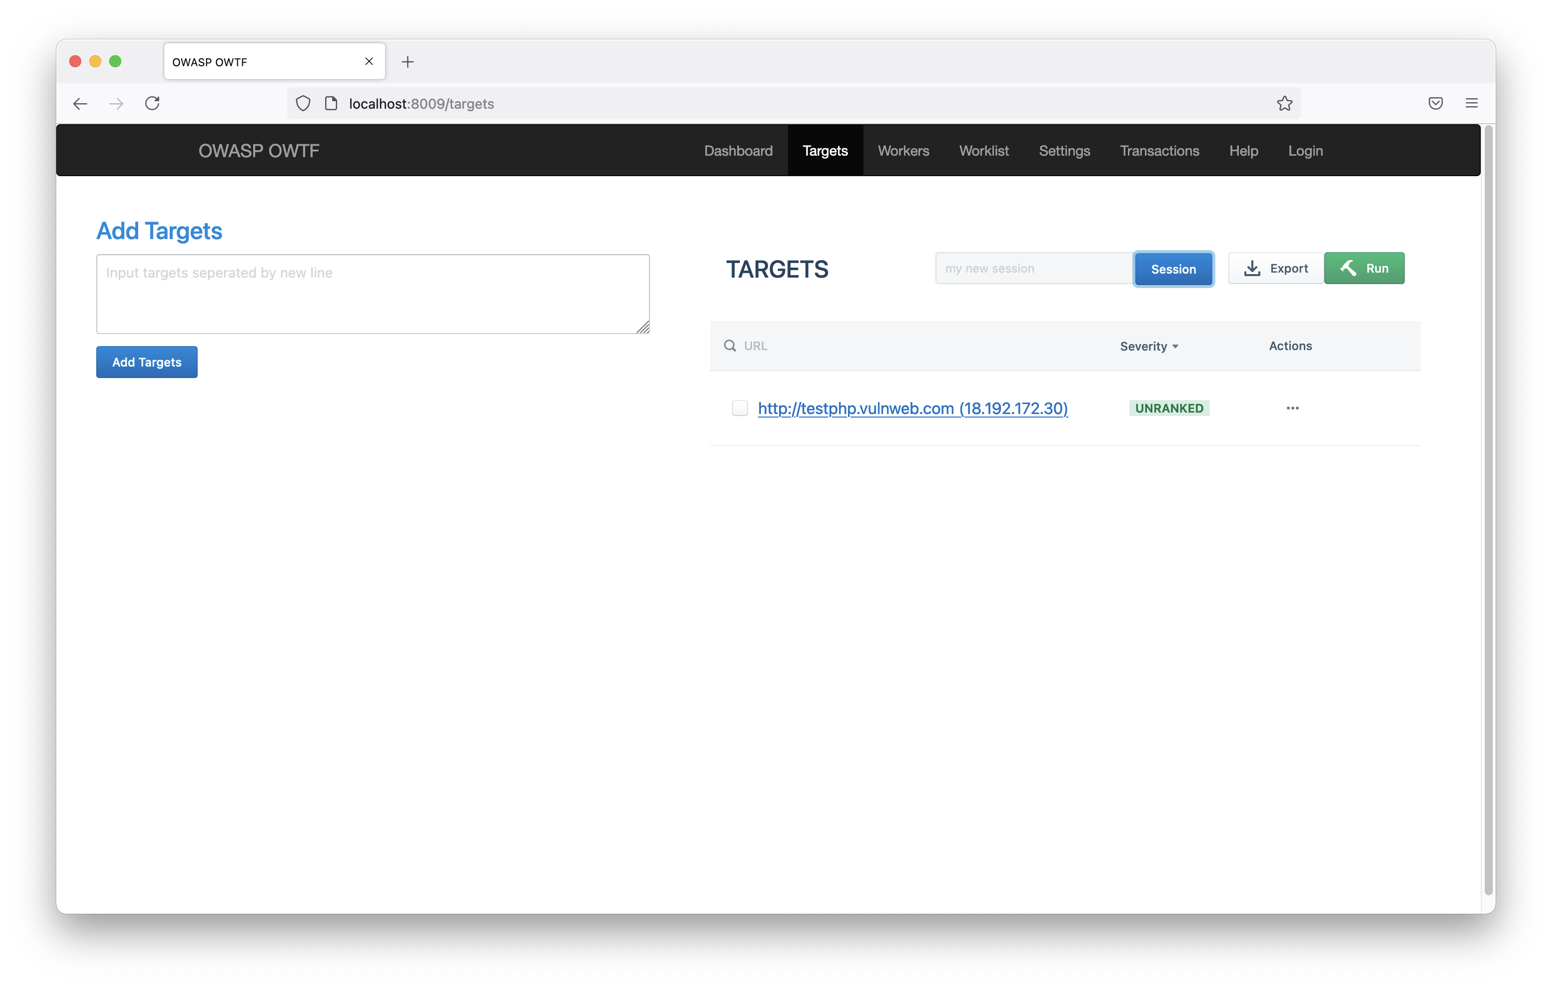
\includegraphics[width=12cm,keepaspectratio=true]{pictures/ui1.png}
	\caption{
		Screenshot of the UI screen after adding a target URL
	}
	\label{fig:ui1}
\end{figure}

Figure \ref{fig:ui1} shows a screenshot of the UI after adding the target URL to our vulnerable target (\textbf{http://testphp.vulnweb.com/} \cite{TestPHP.11.06.2021})), a web application with a vast number of intended security vulnerabilities, developed for educational purposes. As this web application has lots of known vulnerabilities, the author decided to use this application as the target for all further demonstration.

\subsubsection{Selecting and running plugins}

After adding a target, plugins may be started. Plugins have the following structure:\\

\textbf{OWTF-IG-004 Web Application Fingerprint}\\

Under the hood, plugins use command line tools to scan the target(s). For example, the plugin "Web Application Fingerprint" is using curl and whatweb to do its job. The phrase "OWTF-IG-004" is a reference to the OWASP Testing Guide (\cite{Guide.11.06.2021}) and a relation to the chapter "Information gathering" and section "Fingerprint Web Server".

Other plugins like for example \textbf{PTES-001 ftp} reference the Penetration testing execution standard (\cite{PTES.11.06.2021}). Behind the scenes, this plugin uses the "msfconsole" command line tool from the popular metasploit framework.

Figure \ref{fig:ui2} shows the modal window for selecting the plugins to execute against the target. It is possible to launch plugins in groups or individual. On individual selection, text based search is possible to explicitly search for vulnerabilities like "SQL injection" or "Cross site scripting".

\begin{figure}[H]
	\centering
	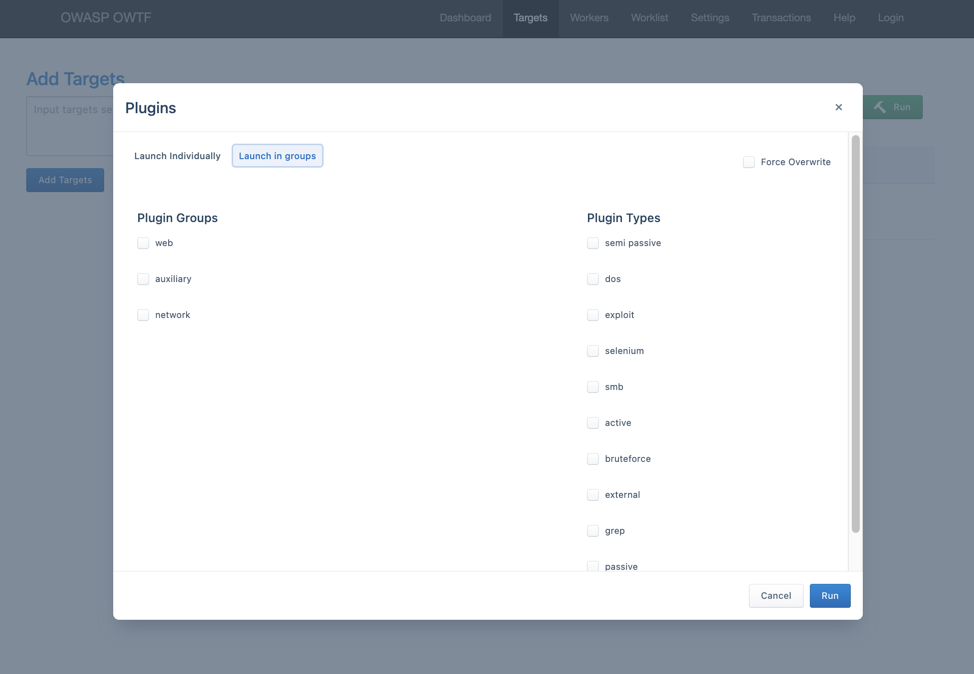
\includegraphics[width=12cm,keepaspectratio=true]{pictures/ui2.png}
	\caption{
		Screenshot of the UI modal window for selecting plugins
	}
	\label{fig:ui2}
\end{figure}

\textbf{Plugin groups}\\

This section explains the plugin groups and types based on the official documentation \cite{OWTFDocs.11.06.2021}.

\begin{itemize}
	\item \textbf{web}\\
	This group contains plugins related basic web capabilities like web application fingerprint or SQL injection
	\item \textbf{auxiliary}\\
	Bruteforce and actual explotation tools
	\item \textbf{network}\\
	Network based scanning tools like DirBuster
\end{itemize}

\textbf{Plugin types}

\begin{itemize}
	\item \textbf{passive}
	\item \textbf{semi passive}
	\item \textbf{active}
	\item \textbf{dos}
	\item \textbf{exploit}
	\item \textbf{selenium}
	\item \textbf{bruteforce}
	\item \textbf{external}
	\item \textbf{grep}
\end{itemize}

First it would be nice to gather some basic information about our target like the IP address, the server on which the site is running on or some information about the framework and tools used by the application. Therefore we start the plugin "OWTF-IG-004 Web Application Fingerprint", which uses "whatweb" and "curl" under the hood.

\subsubsection{Report page - analyzing the scan results}

In Figure \ref{fig:ui3} the detail page of a target after running the fingerprint plugin is shown. The left sidebar provides options for filtering plugin results based on plugin groups and plugin types and generating and downloading the final report. In the middle, run plugins are rendered including the plugin type and the title of the plugin. Clicking on one of the plugins opens a flyover window on the right of the screen for viewing the plugin output or adding custom notes. It is possible to categorize the plugin in the following states: \textbf{Unranked}, \textbf{Passing}, \textbf{Info}, \textbf{Low}, \textbf{Medium}, \textbf{High} and \textbf{Critical}. This is helpful for filtering later and to better organize our work. Clicking on the \textbf{Browse} button opens the results of the scan in a new window.

\begin{figure}[H]
	\centering
	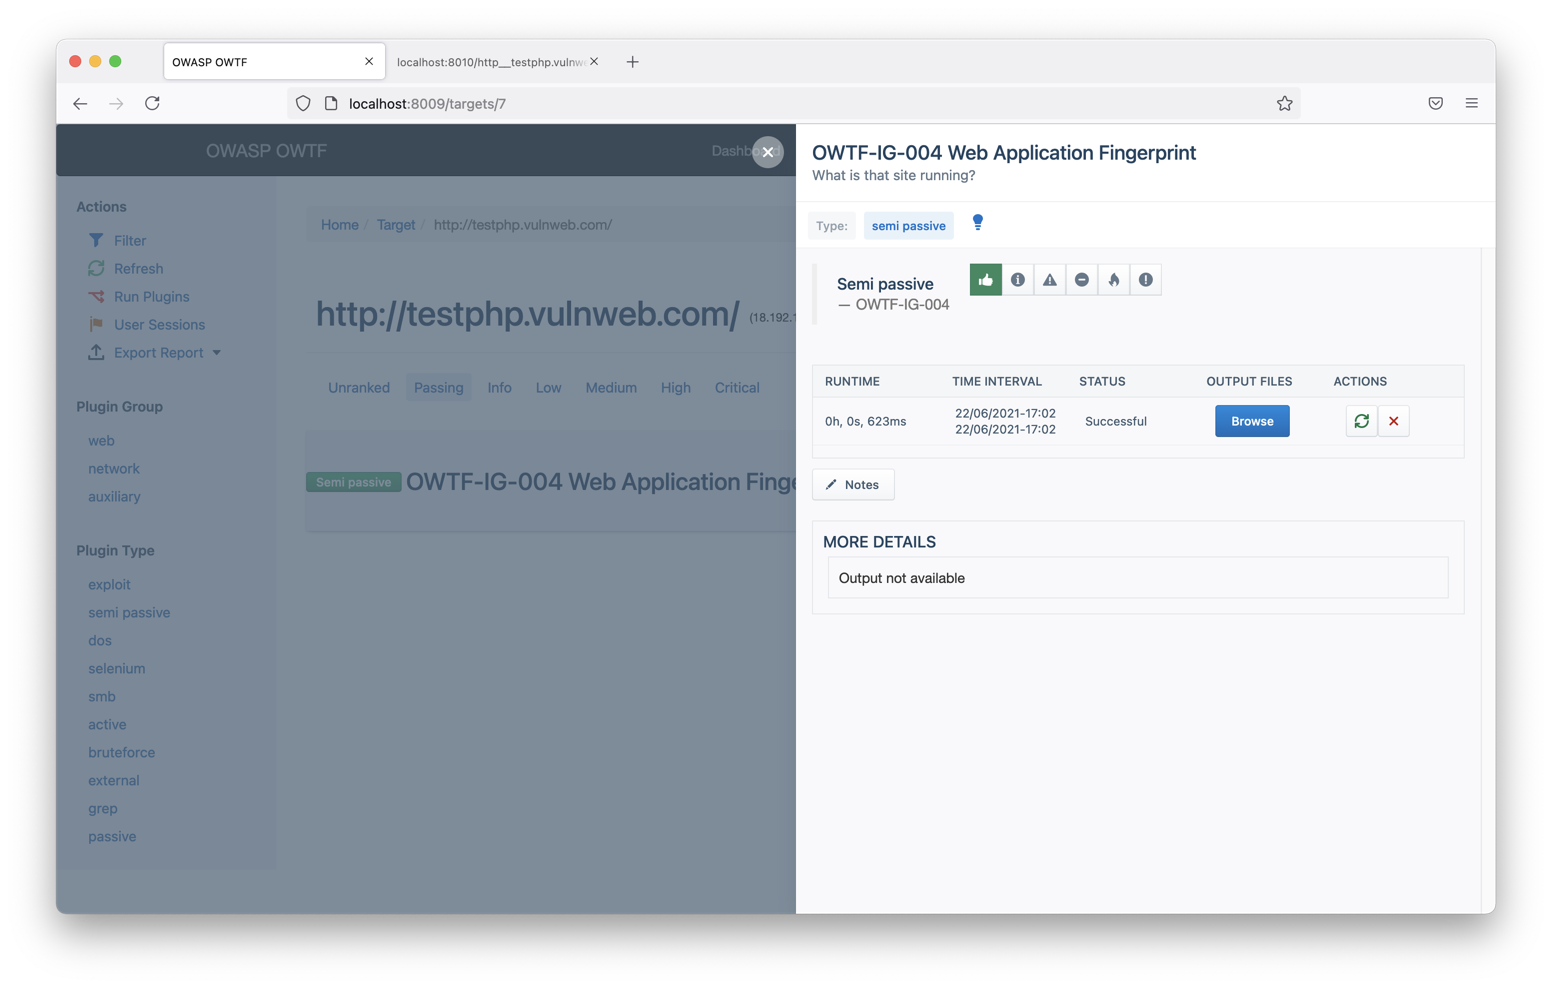
\includegraphics[width=12cm,keepaspectratio=true]{pictures/ui3.png}
	\caption{
		Screenshot of the UI page of a target after running the plugin "Web Application Fingerprint"
	}
	\label{fig:ui3}
\end{figure}

The result of the underlying "whatweb" command looks like this:

\begin{verbatim}
http://testphp.vulnweb.com/ [200 OK] ActiveX[D27CDB6E-AE6D-11cf-96B8-444553540000]
Adobe-Flash, Country[UNITED STATES][US]
Email[wvs@acunetix.com]
HTTPServer[nginx/1.19.0]
IP[18.192.172.30]
Object[http://download.macromedia.com/...
PHP[5.6.40-38+ubuntu20.04.1+deb.sury.org+1]
Script[text/JavaScript]
Title[Home of Acunetix Art]
UncommonHeaders[x-http-reason]
X-Powered-By[PHP/5.6.40-38+ubuntu20.04.1+deb.sury.org+1]
nginx[1.19.0]
\end{verbatim}

So among other information, this tells us that the site is served by an nginx server in version 1.19.0, it runs on PHP 5.6.40 and it is using JavaScript. Looks like a regular web application, so we are going to try some active vulnerability scanning. We select the plugin \textbf{OWTF-WVS-006 Skipfish Unauthenticated}. The plugin unfortunately runs into an error, but it tells us which command it wants to run. We now want to try the command manually.

\subsubsection{Running and analyzing CLI commands}

We open a terminal inside the docker container with the following command:

\begin{lstlisting}
$ docker exec -it docker_owtf_1 bash
\end{lstlisting}

Now that we have a shell inside the kali linux docker container we can execute the commands just like \ac{owtf} would. After some tweaking we try the following:

\begin{lstlisting}
touch new_dict.wl
skipfish -t 90 -i 90 -w 90 -f1000 -b f -o /tmp/skip -W ./new_dict.wl http://testphp.vulnweb.com
\end{lstlisting}

Figure \ref{fig:terminal1} shows a screenshot of the command terminal output.

\begin{figure}[H]
	\centering
	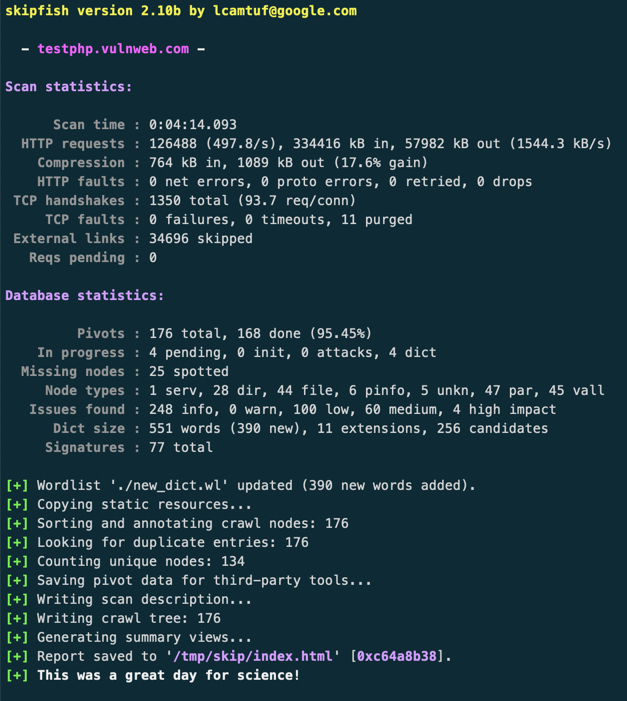
\includegraphics[width=12cm,keepaspectratio=true]{pictures/terminal1.png}
	\caption{
		Screenshot of the Terminal output of the skipfish command
	}
	\label{fig:terminal1}
\end{figure}

After the command run, it generated an html report which we download to our host for inspection. Figure \ref{fig:ui4} shows a screenshot of the report.

\begin{figure}[H]
	\centering
	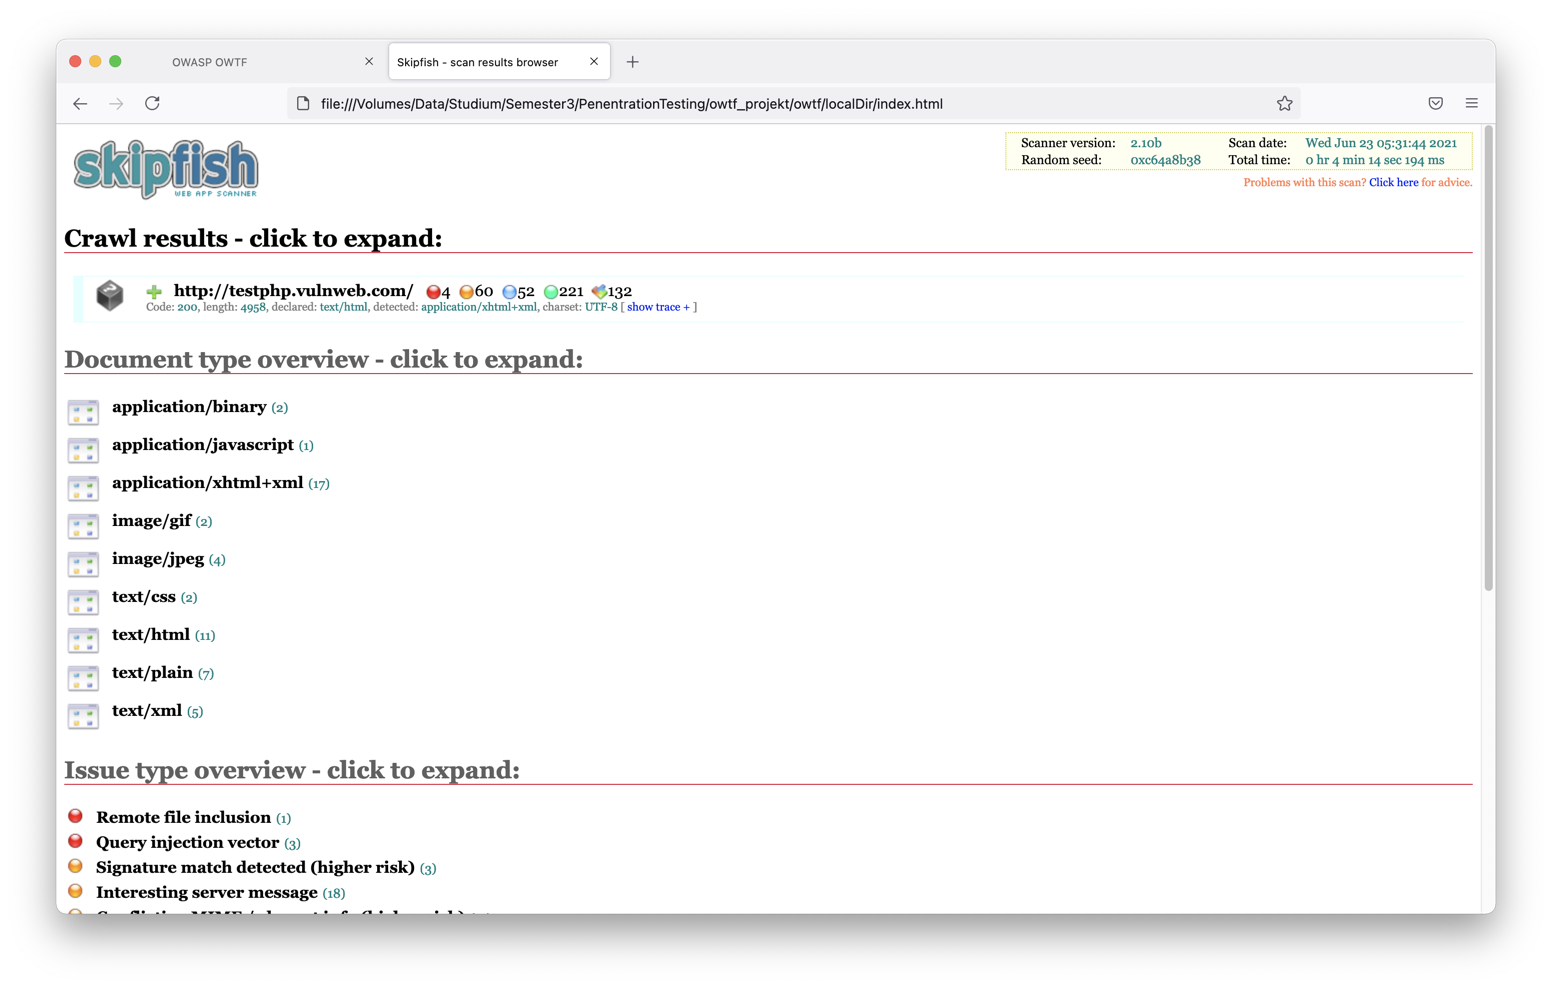
\includegraphics[width=12cm,keepaspectratio=true]{pictures/ui4.png}
	\caption{
		Screenshot of the skipfish report
	}
	\label{fig:ui4}
\end{figure}

Analyzing the report we see 16 XSS vectors. The web application allows users to list products filtering for a category. The parameter payload for the URL \textbf{http://testphp.vulnweb.com/listproducts.php} looks like this:

\begin{verbatim}
?cat=%22.$.htaccess.aspx--%3E%22%3E%27%3E%27%22%3Csfi000107v352075%3E
\end{verbatim}

Navigating to that URL renders a MySQL exception, which is a hint that we may inject code:

\begin{verbatim}
Error: You have an error in your SQL syntax; check the manual that 
corresponds to your MySQL server version for the right syntax to 
use near '"' at line 1 Warning: mysql_fetch_array() expects 
parameter 1 to be resource, boolean given in 
/hj/var/www/listproducts.php on line 74 
\end{verbatim}

After some manual playing with this payload we found a working reflected XSS injection using the following payload:

\begin{lstlisting}[breaklines]
?cat=".$.htaccess.aspx-->">'>'"<script>alert('OK')</script>
\end{lstlisting}

Here is a link to the full working exploit URL: 
\href{http://testphp.vulnweb.com/listproducts.php?cat=".$.htaccess.aspx-->">'>'"<script>alert('OK')</script>}{Link}\\

Figure \ref{fig:ui5} shows a screenshot of the successful exploit.

\begin{figure}[H]
	\centering
	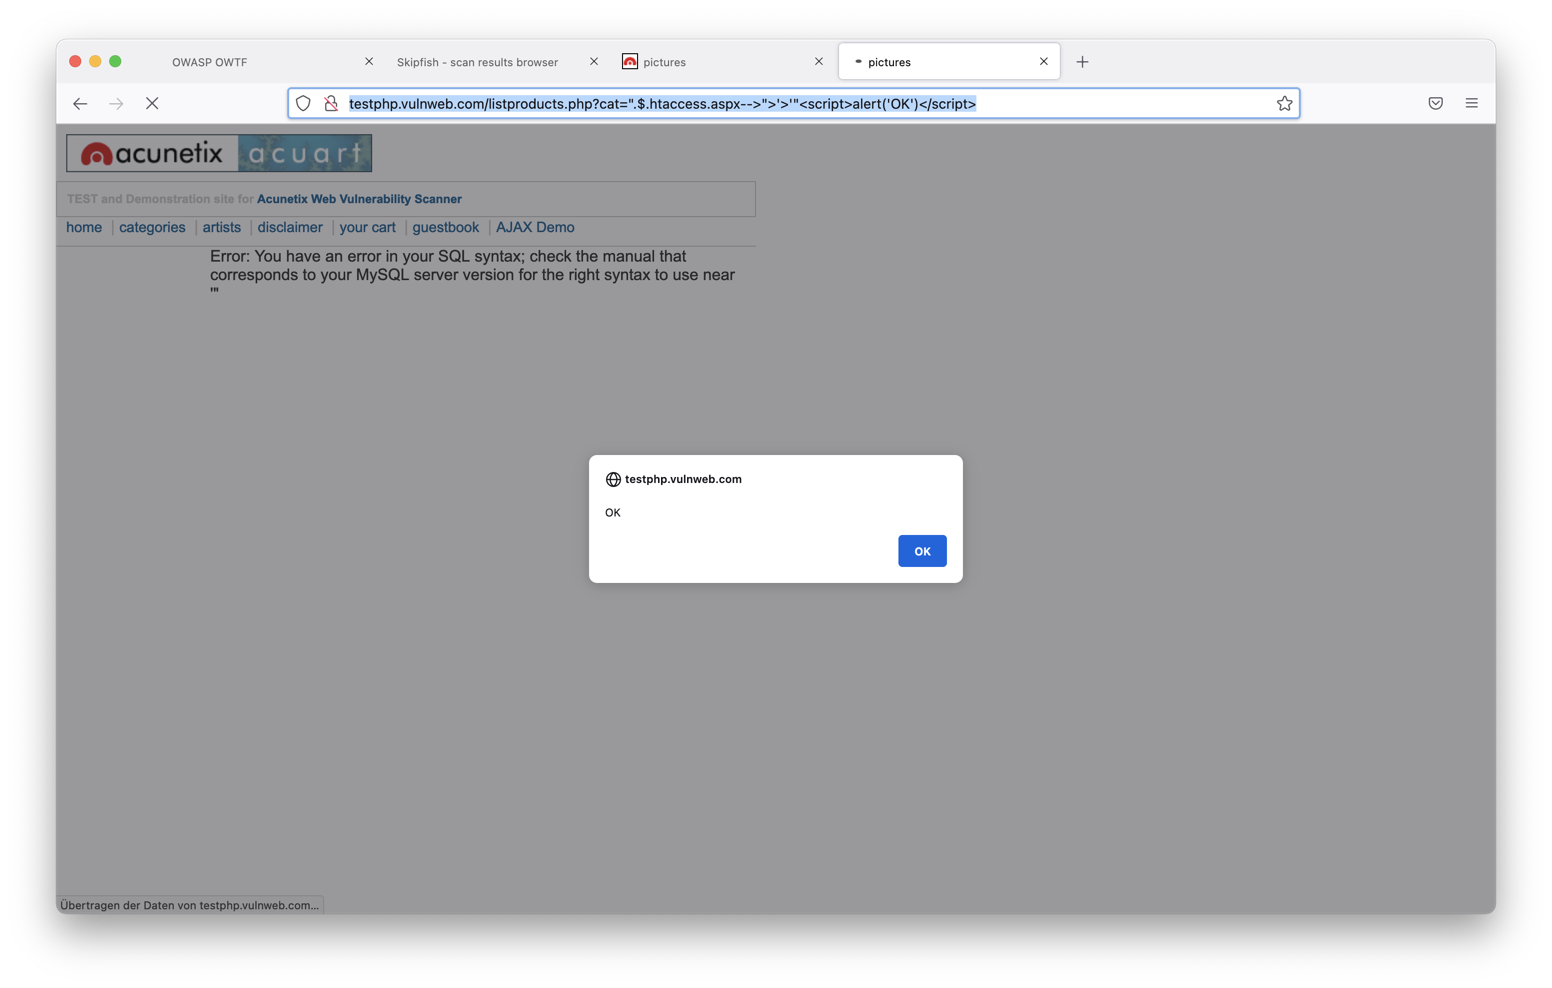
\includegraphics[width=12cm,keepaspectratio=true]{pictures/ui5.png}
	\caption{
		Successful exploit of a reflected XSS vector
	}
	\label{fig:ui5}
\end{figure}

\subsubsection{Adding notes in the web UI}

Now that we found a successful exploit we go back to the user interface and add some notes to our plugin and categorize the plugin run as critical. See Figure \ref{fig:ui6} for a detailed screenshot.

\begin{figure}[H]
	\centering
	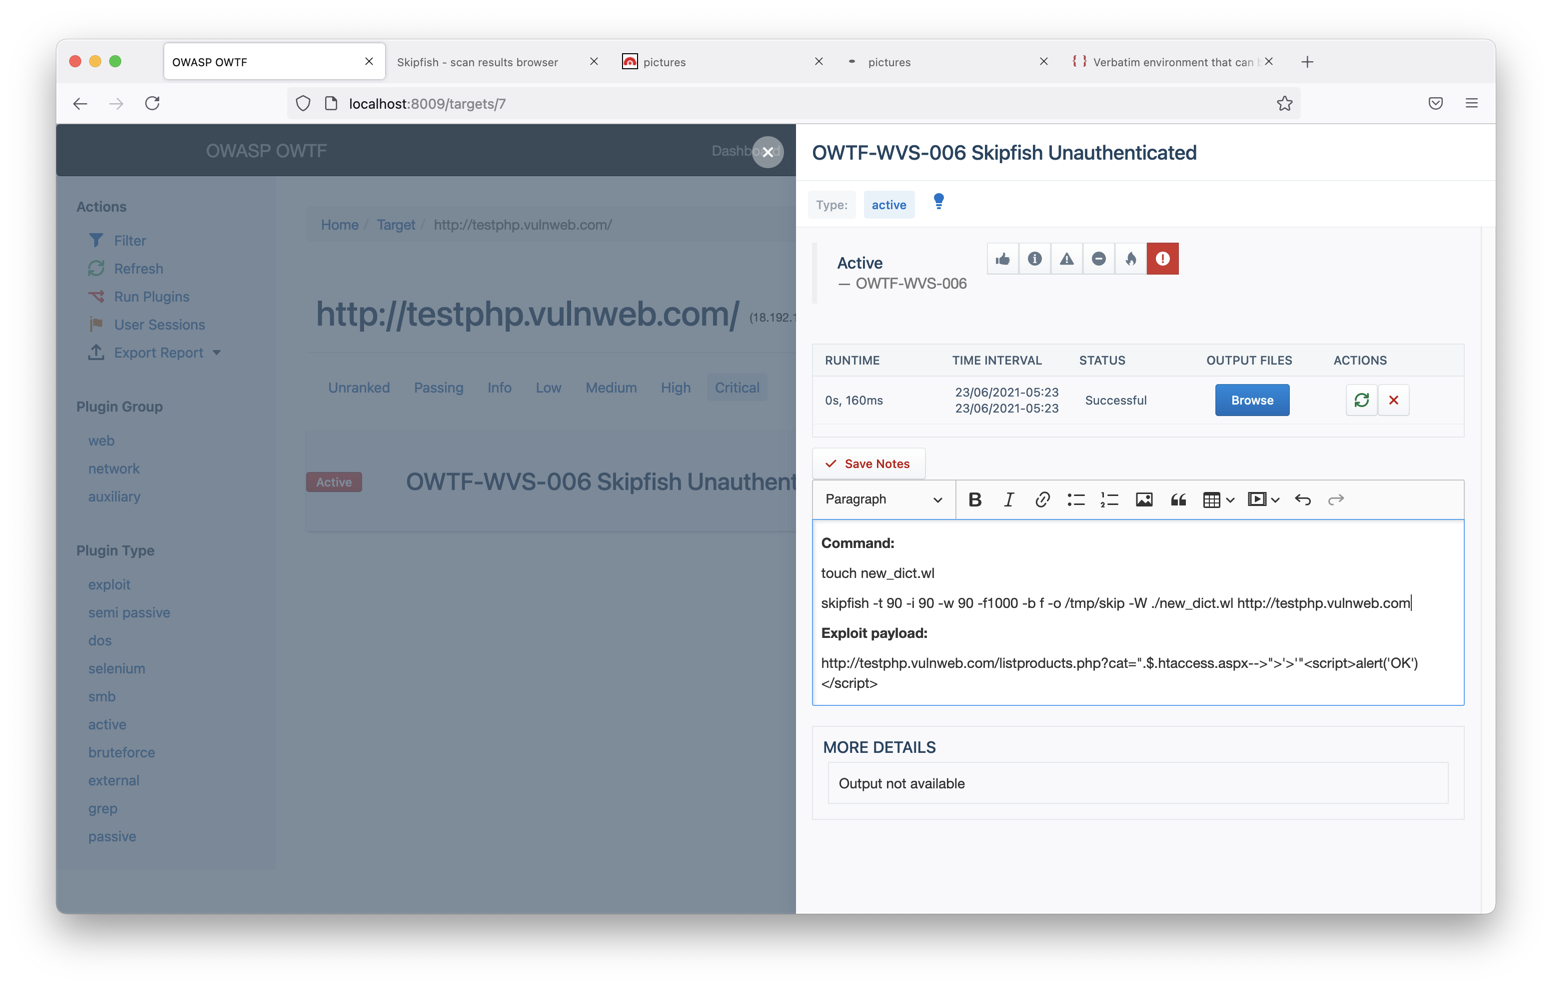
\includegraphics[width=12cm,keepaspectratio=true]{pictures/ui6.png}
	\caption{
		Screenshot of adding manual notes to a plugin
	}
	\label{fig:ui6}
\end{figure}

\subsubsection{Generating (export) the report}

Unfortunatly, exporting the report seems to be broken. After some analysis of the inner workings, an issue on GitHub was created by the author:\\\\ \href{https://github.com/owtf/owtf/issues/1149}{https://github.com/owtf/owtf/issues/1149}

\subsubsection{Dashboard}

Finally we take a look at the dashboard which could also be very helpful for reporting our work. Figure \ref{fig:ui7} shows a screenshot of the dashboard. As seen in the screenshot, the used categorization inside the plugin views are represented here in a nice looking chart.

\begin{figure}[H]
	\centering
	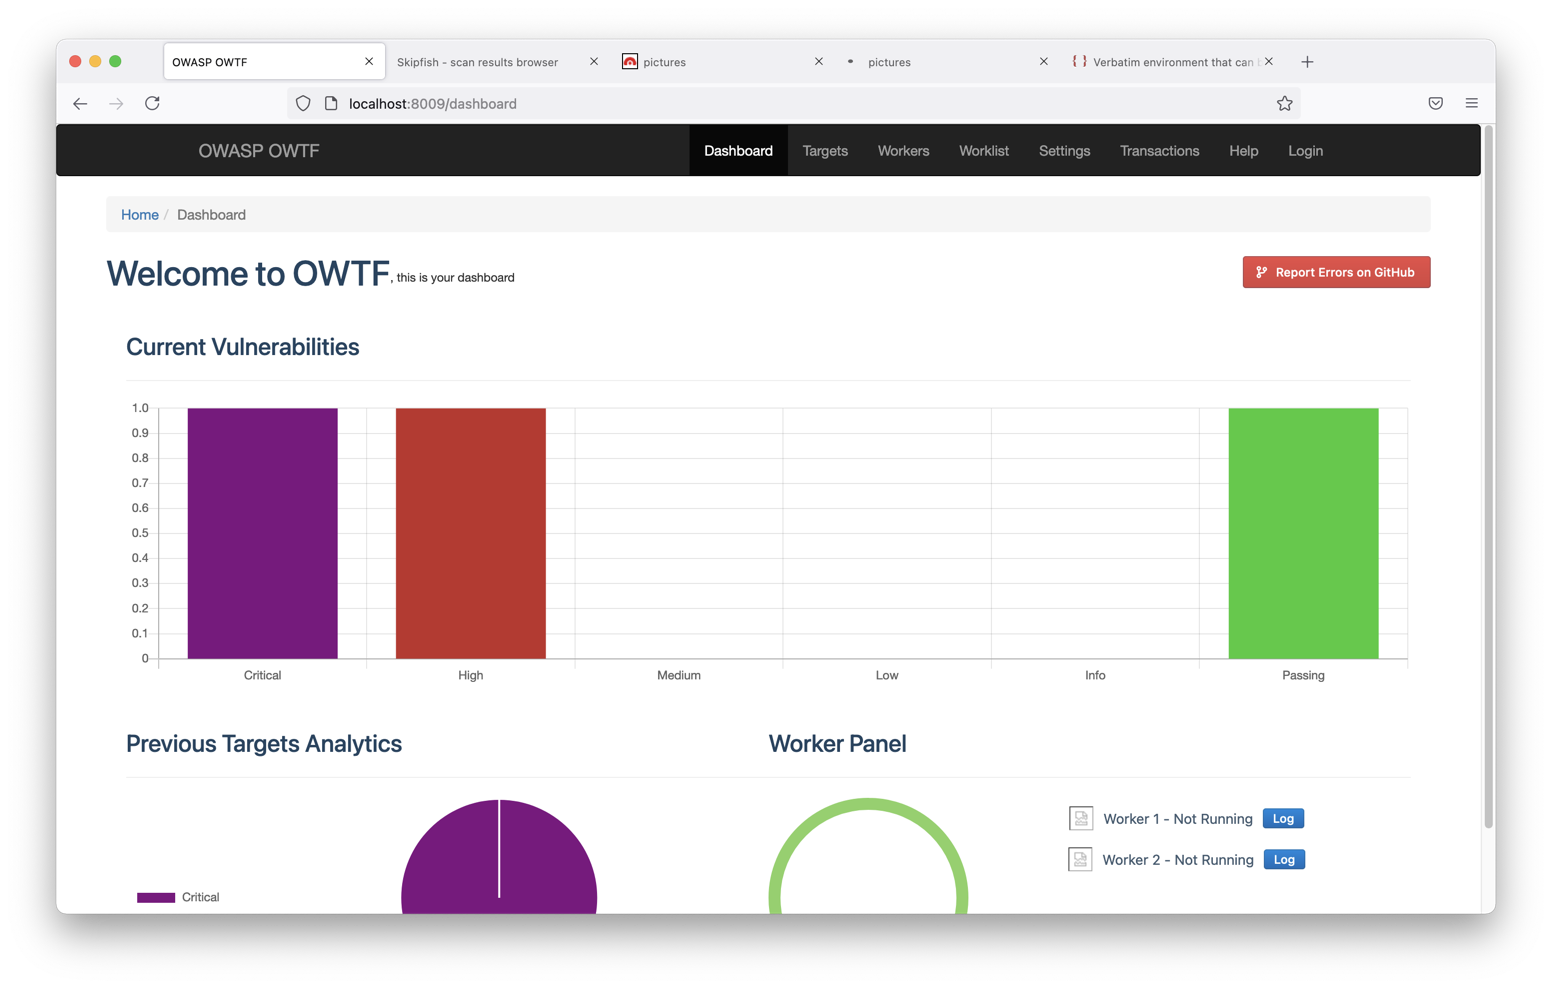
\includegraphics[width=12cm,keepaspectratio=true]{pictures/ui7.png}
	\caption{
		Screenshot of the dashboard
	}
	\label{fig:ui7}
\end{figure}

\newpage

\section{Conclusion}

The first impression of the tool including its motivation, goals and features looked really impressive. Having a tool supporting the complete process of penetration testing, aligned to security standards and containing support for automatic report generation really could enhance the life of a security tester. Setup and installation was quite simple and pretty straightforward. Supporting a docker based installation deserves some bonus points too.
But after exploring and trying to use the tool in a productive way, the overall experience was pretty disappointing.

Lots of features just don't work as expected and are running into an error. The following list gives an overview and documents the author's findings:

\begin{itemize}
	\item \textbf{Starting plugins}\\
	Starting plugins, especially multiple at the same time or in groups, randomly leads to an error with the message "Unable to add Error: Bad Request". The POST request returns a status code 400 Bad Request with the error "Plugin list should not be empty", even though the checkboxes for selecting plugin (groups) was selected before clicking the "Run" button.
	\item \textbf{Looking at the plugin results}\\
	Looking at the plugin results is not possible in some cases. Clicking on the "Browse" button to view a plugins' results navigates to an URL like \textbf{http://localhost:8010/null/} with a status code 404 Not Found.
	\item \textbf{Report generation and download}\\
	Clicking on the "Export Report" button leads to a white screen and a JavaScript error in the DevTools console saying "The menu has no menu items". An issue at the git repository on GitHub was created by the author: \href{https://github.com/owtf/owtf/issues/1149}{https://github.com/owtf/owtf/issues/1149}
	\item \textbf{Tools not found}\\
	Sometimes when running a plugin, the tools does not seem to be installed inside the docker based virtual machine (e.g. theHarvester: command not found)
\end{itemize}

Nevertheless it should be kept in mind that \ac{owtf} is a free, open source solution containing lots of work (the repository was created in January 2012), as can be seen looking at the git source repository history. 
Also, it is under active development and there is a web page for addressing and optimizing some pain points in the context of the google summer of code 2021 \cite{GSoC2021.11.06.2021}. For example they want to enhance the user experience and are searching for developers implementing some overall improvements. The author had some discussion on the development slack channel and the maintainers responded quickly, were thankful for reporting these issues and want to address them very soon.

Finally, in the opinion of the author, at current stage there are too many issues and lots of debugging needed, so the tool just not seem to be ready for production use. But as the tool is still under active development, is is possible that the contributors add more documentation and fix the found issues in the foreseeable future and it is definitely worth \textbf{\href{https://twitter.com/owtfp/}{following}} the development of this promising solution.
